\subsection{Pooling} \label{subs:pooling}
A Pooling layer is used to replace the output of the previous layer by a summary statistics of this output \cite{goodfellow_deep_2016}. They are usually inserted between the successive convolutional layer to modify the output further. Its goal is first to make the output approximately invariant to small translations and it also reduces the spatial size of each output \acrshort{fm}. It means that the memory needed to store the parameters is reduced \cite{goodfellow_deep_2016}. It also reduces the number of parameters and the computation of the network while also increasing the receptive field \cite{shawahna_fpga-based_2019}.

The pooling layer divides each \acrshort{fm} into regions of size $K \title K$ and outputs one pixel from each region. This way, is kept constant while their spatial size is reduced by $K$. Various pooling functions exist, but the most common form uses filters of size $2 \times 2$ where for example the MAX or AVG operation selects the highest pixel from 4 samples their average respectively (meaning a 75\% reduction of the pixels) \cite{suda_throughput-optimized_2016}. Figure \ref{fig:pool} illustrates an example of a pooling layer.
%
\begin{figure}
    \centering
    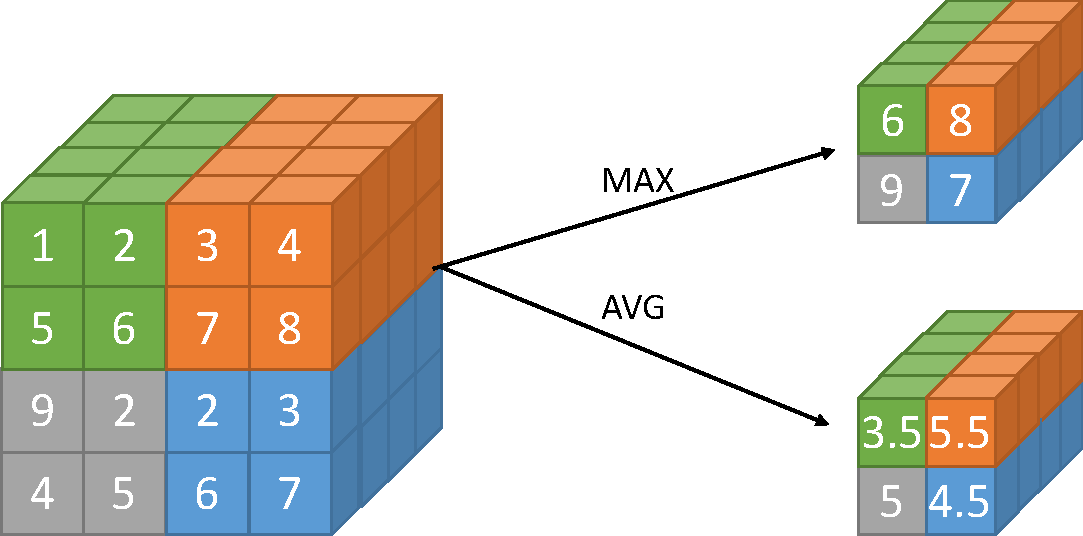
\includegraphics[width=0.8\textwidth]{pooling.pdf}
    \caption{An example of pooling layers}
    \label{fig:pool}
\end{figure}
